\documentclass{jarticle}

\usepackage{graphicx}
\usepackage{url}
\usepackage{listings,jlisting}
\usepackage{ascmac}
\usepackage{amsmath,amssymb}

%ここからソースコードの表示に関する設定
\lstset{
  basicstyle={\ttfamily},
  identifierstyle={\small},
  commentstyle={\smallitshape},
  keywordstyle={\small\bfseries},
  ndkeywordstyle={\small},
  stringstyle={\small\ttfamily},
  frame={tb},
  breaklines=true,
  columns=[l]{fullflexible},
  numbers=left,
  xrightmargin=0zw,
  xleftmargin=3zw,
  numberstyle={\scriptsize},
  stepnumber=1,
  numbersep=1zw,
  lineskip=-0.5ex
}
%ここまでソースコードの表示に関する設定

\title{知能プログラミング演習II 課題4}
\author{グループ07\\
  29114007 池口 弘尚\\
%  {\small (グループレポートの場合は、グループ名および全員の学生番号と氏名が必要)}
}
\date{2019年10月28日}

\begin{document}
\maketitle

\paragraph{提出物} rep4
\paragraph{グループ} グループ07
\paragraph{メンバー}
\begin{tabular}{|c|c|c|}
  \hline
  学生番号&氏名&貢献度比率\\
  \hline\hline
  29114007&池口弘尚&\\
  \hline
  29114031&大原拓人&\\
  \hline
  29114048&北原太一&\\
  \hline
  29114086&飛世裕貴&\\
  \hline
  29114095&野竹浩二朗&\\
\end{tabular}

\section{課題の説明}
\begin{description}
\item[課題4-1] まず,教科書3.2.1の「前向き推論」のプログラムと教科書3.2.2の「後向き推論」のプログラムとの動作確認をし,前向き推論と後ろ向き推論の違いを説明せよ.また,実行例を示してルールが選択される過程を説明せよ.説明の際には,LibreOfficeのDraw(コマンド soffice --draw)などのドロー系ツールを使ってp.106 図3.11やp.118 図3.12のような図として示すことが望ましい.
\item[課題4-2] CarShop.data , AnimalWorld.data 等のデータファイルを実際的な応用事例(自分達の興味分野で良い)に書き換えて,前向き推論,および後ろ向き推論に基づく質問応答システムを作成せよ.どのような応用事例を扱うかは,メンバーで話し合って決めること.
 なお,ユーザの質問は英語や日本語のような自然言語が望ましいが,難しければ変数を含むパターン等でも可とする.
\item[課題4-3] 上記4-2で実装した質問応答システムのGUIを作成せよ.
 質問に答える際の推論過程を可視化できることが望ましい.
\item[課題4-4]上記4-3で実装したGUIを発展させ,質問応答だけでなく,ルールの編集(追加,削除,変更)などについてもGUIで行えるようにせよ.
\end{description}
私は課題4-3と課題4-4を担当した。

\section{課題4-3}
\begin{screen}
 上記4-2で実装した質問応答システムのGUIを作成せよ.
 質問に答える際の推論過程を可視化できることが望ましい.
\end{screen}

\subsection{手法}
課題4-2で作成した探索をカプセル化し、GUI側からそれを呼び出すことによって実装した。

\subsection{実装}
基本的な構造は今までと同じなので省略する。
今回で新たに使用したのは、JTextFieldでエンターを押したときの判定の取り方である。

\begin{lstlisting}[caption=JTextFieldのActionListener,label=src:text]
public ForwardSearchPanel(String name, kadai4.ForwardChain.RuleBaseSystem rbs) {
	(略)
	ActionListener searchActionListener = new ActionListener() {
		@Override
		public void actionPerformed(ActionEvent e) {
			rbs.patternSearch(text1.getText());
			text1.setText("");
		}
	};
	text1.addActionListener(searchActionListener);
	button.addActionListener(searchActionListener);
}
\end{lstlisting}
上のコードのように今までボタンに付けていたActionListenerをJTextFieldにも加えることによって、入力のわずらわしさを減らすことができた。

また、今回はそれぞれのパネルをJTabbedPaneを使用してタブで分けた。
そのために今まで使ってきたFrameBaseを継承してPageFrameBaseを以下のように作成した。
\begin{lstlisting}[caption=PageFrameBase,label=src:PageFrameBase]
public class PageFrameBase extends FrameBase {
	JTabbedPane tabbedpane;

	public PageFrameBase(String title, int x, int y, int width, int height, PagePanelBase[] pages) {
		super(title, x, y, width, height);
		MakePages(pages);
	}

	public PageFrameBase(String title, int width, int height, PagePanelBase[] pages) {
		super(title, width, height);
		MakePages(pages);
	}
	//ページを作成
	private void MakePages(PagePanelBase[] pages) {
		JPanel p = new JPanel();

		tabbedpane = new JTabbedPane();
		for (PagePanelBase Panel : pages) {
			tabbedpane.add(Panel, Panel.getName());
		}
		//tabbedpane.setSize(1600, 100);

		LogArea logArea = new LogArea(30, 140);
		SpringLayout layout = new SpringLayout();
		p.setLayout(layout);

		layout.putConstraint(SpringLayout.NORTH, tabbedpane, 5, SpringLayout.NORTH, p);
		layout.putConstraint(SpringLayout.SOUTH, tabbedpane, 305, SpringLayout.NORTH, p);
		layout.putConstraint(SpringLayout.EAST, tabbedpane, -30, SpringLayout.EAST, p);
		layout.putConstraint(SpringLayout.WEST, tabbedpane, 30, SpringLayout.WEST, p);

		layout.putConstraint(SpringLayout.NORTH, logArea, 10, SpringLayout.SOUTH, tabbedpane);
		layout.putConstraint(SpringLayout.HORIZONTAL_CENTER, logArea, 0, SpringLayout.HORIZONTAL_CENTER, p);

		p.add(tabbedpane);
		p.add(logArea);
		add(p, BorderLayout.CENTER);
	}

}
\end{lstlisting}
PagePanelBaseはJPanelに名前を持たせただけのクラスなので説明は省く。

課題2の時にはそれぞれのログは別で表示されていたが、今回はPageFrameBaseでログエリアを作成することによって共通で使えるようにしてある。
また、今回の課題では過程を表示しなければならないため、どこからでもログを表示できる必要があった。
そのため、LogAreaは以下のように実装した。

\begin{lstlisting}[caption=Log,label=src:log]
public class LogArea extends JScrollPane {
	static LogArea instance;
	JTextArea area;
	JViewport viewport;

	public LogArea(int rows, int columns) {
		super();
		area = new JTextArea(rows, columns);
		EtchedBorder border = new EtchedBorder(EtchedBorder.RAISED);
		area.setEditable(false);
		area.setBorder(border);
		setViewportView(area);
		viewport = getViewport();
		instance = this;
	}
	//1行ログを表示
	public static void println(String txt) {
    	//インスタンスが無ければSystem.out
		if (instance != null)
			instance.area.append(txt + "\n");
		else
			System.out.println(txt);
	}
	//続けてログを表示
	public static void print(String txt) {
    	//インスタンスが無ければSystem.out
		if (instance != null)
			instance.area.append(txt);
		else
			System.out.print(txt);
	}
}
\end{lstlisting}
これは、GUIが作成されていなければSystem.outが使われるため、作業段階から利用することができる。

\subsection{実行例}
\begin{figure}[!hbt]
  \centering
  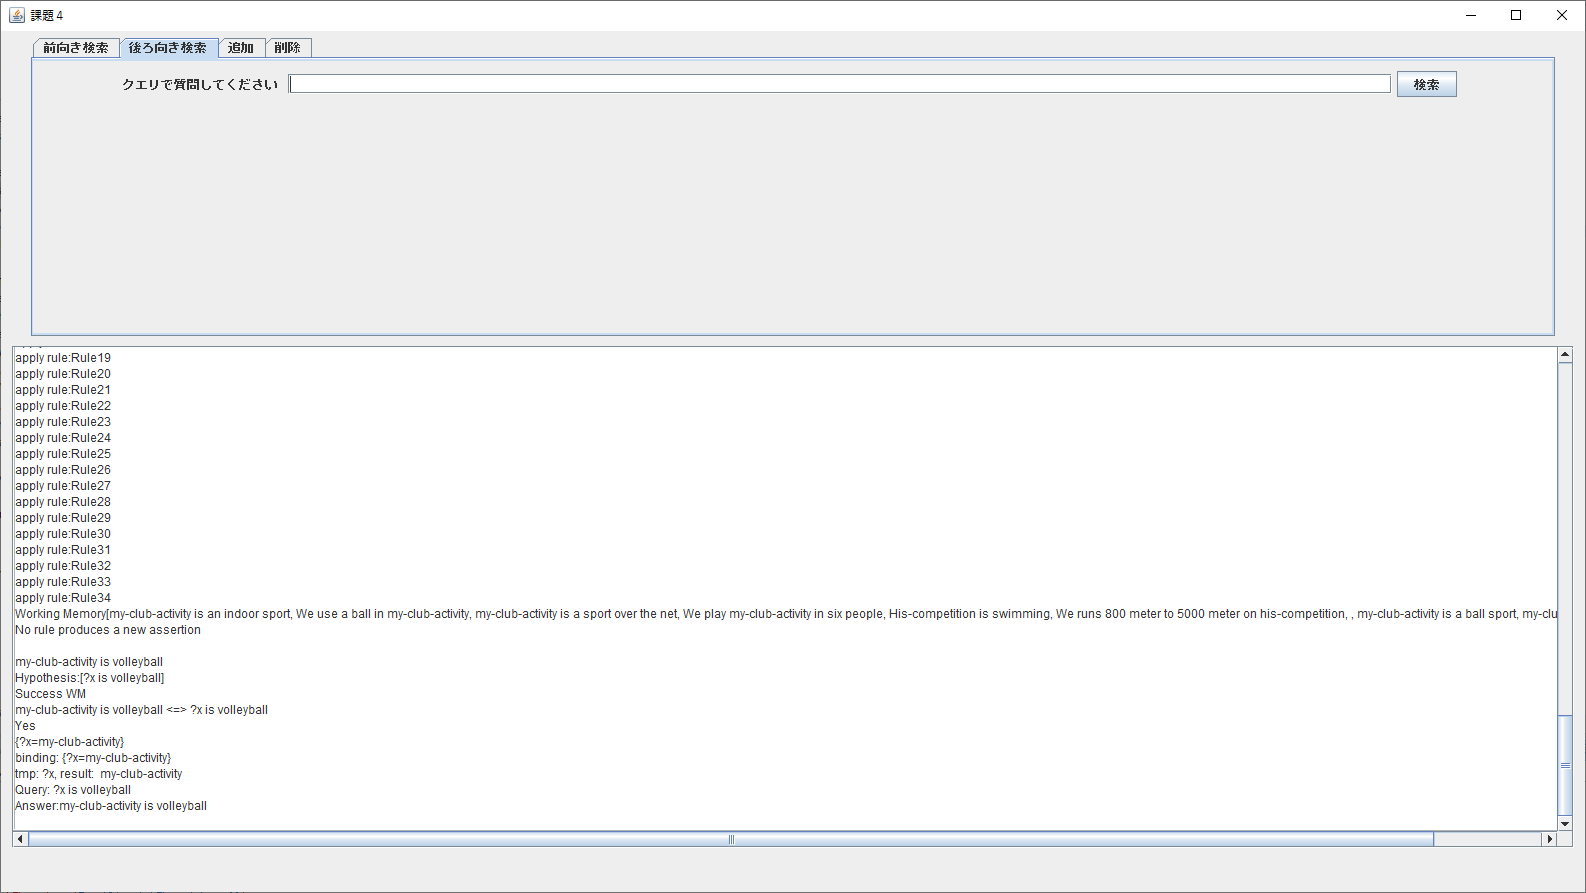
\includegraphics[bb=0 0 1586 893,width=1.2\linewidth]{GUI1.png}
  \caption{検索例}
  \label{fig:Search}
\end{figure}
\subsection{考察}
外側のメソッドを呼ぶだけなので問題は生じなかった。

\section{課題4-4}
\begin{screen}
 上記4-3で実装したGUIを発展させ,質問応答だけでなく,ルールの編集(追加,削除,変更)などについてもGUIで行えるようにせよ.
\end{screen}

\subsection{手法}
今までと同様な手法によってGUIに追加する。
変更に関しては、削除してから新たに追加することとした。
\subsection{実装}
GUI部分に関しては今までと変わらないため説明は省く。
RuleBase部分を編集してルールの追加などを行えるようにした。
\begin{lstlisting}[caption=編集,label=src:Change]
//ルールを1つ追加
public void addRules(String name, ArrayList<String> antecedents, String consequent) {
	rules.add(new Rule(name, antecedents, consequent));
}
//ルール名で削除
public void deleteRules(String name) {
	for (int i = 0; i < rules.size(); i++) {
		if (rules.get(i).getName().equals(name)) {
			LogArea.println("Delete:" + rules.get(i));
			rules.remove(i);
			i--;
		}
	}
}
//アサーションを削除
public void deleteAssertion(String assertion) {
	wm.assertions.remove(assertion);
}
//ルールをまとめて追加
public void addRules(List<Rule> rules) {
	for (Rule rule : rules) {
		if (!this.rules.contains(rule)) {
			LogArea.println("Add:" + rule);
			this.rules.add(rule);
		}
	}
}
//アサーションをまとめて追加
public void addWorkingMemory(List<String> wmlist) {
	for (String string : wmlist) {
		wm.addAssertion(string);
	}
}
//アサーションを1つ追加
public void addWorkingMemory(String wmline) {
	wm.addAssertion(wmline);
}
\end{lstlisting}

\newpage
\subsection{実行例}
\begin{figure}[!hbt]
  \centering
  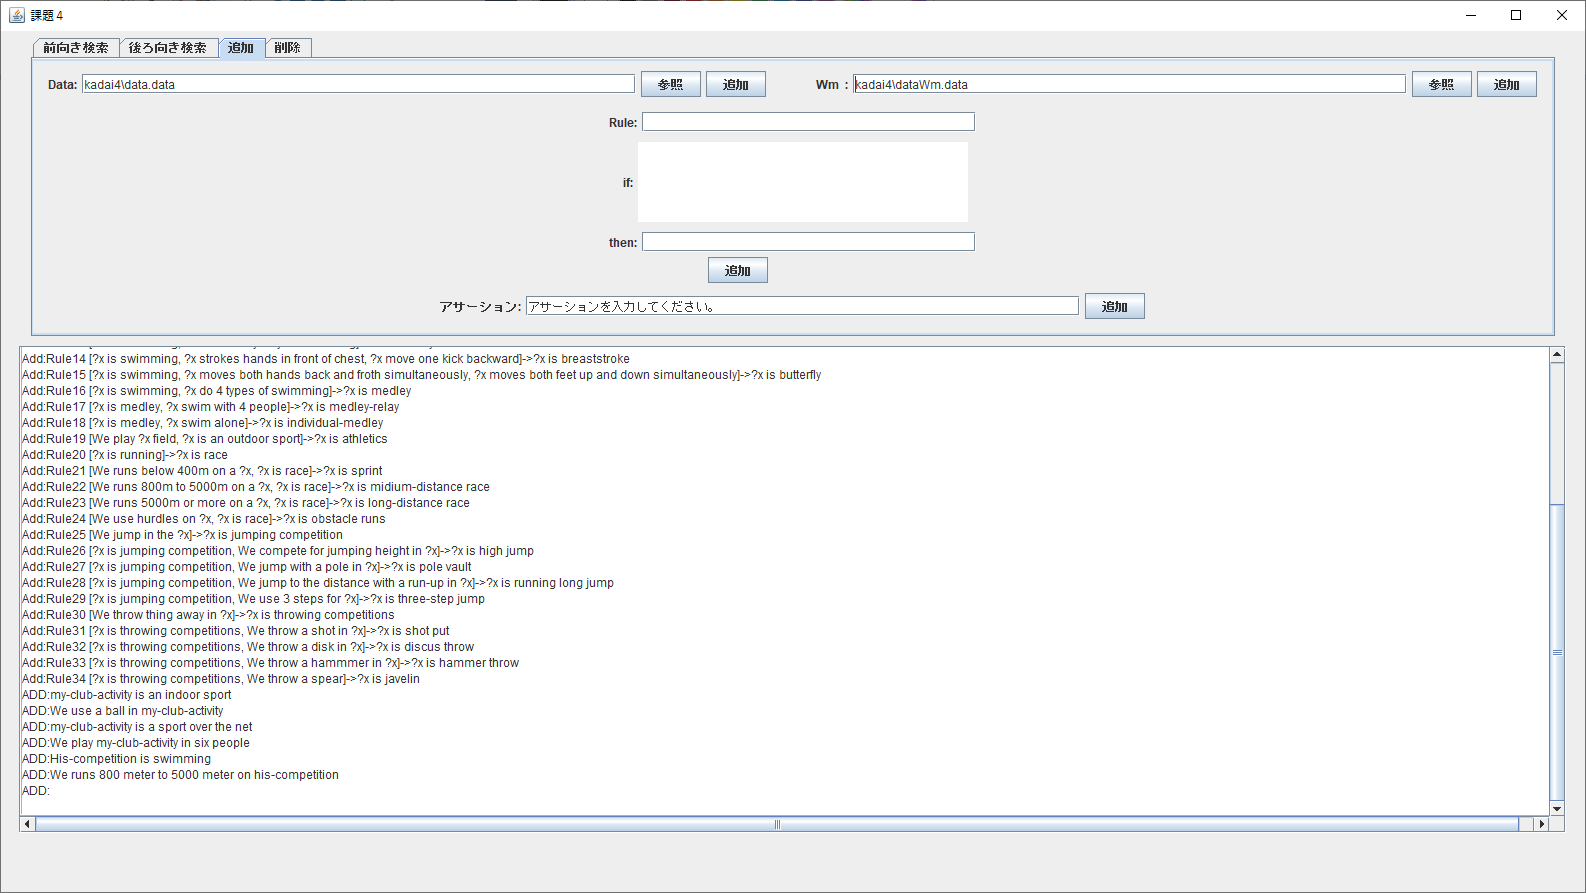
\includegraphics[bb=0 0 1586 893,width=1.2\linewidth]{GUI2.png}
  \caption{追加例}
  \label{fig:Add}
  \centering
  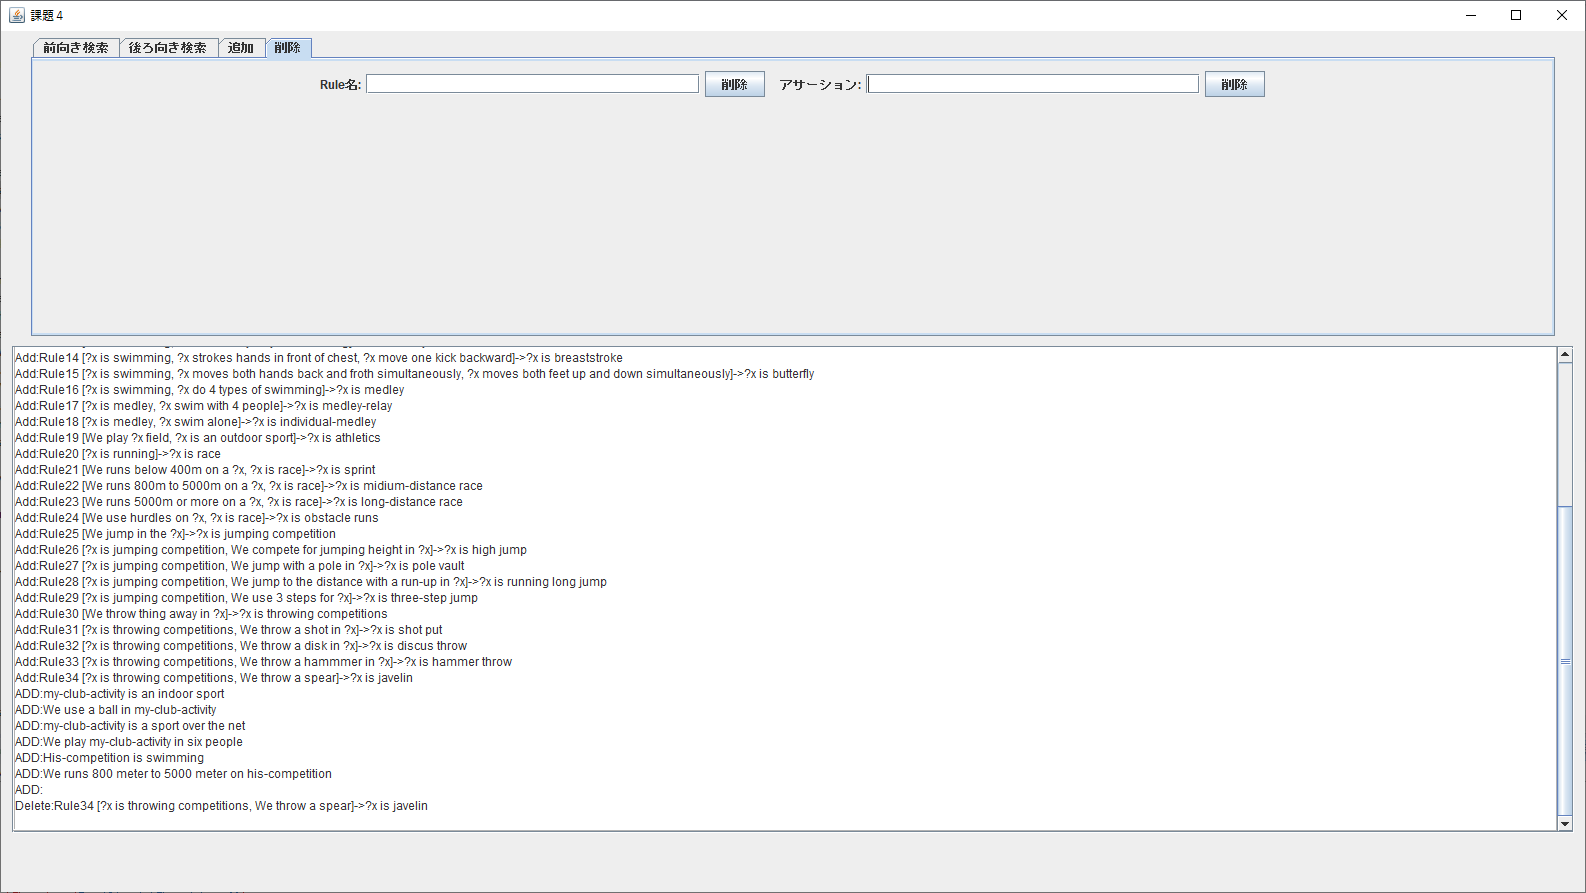
\includegraphics[bb=0 0 1586 893,width=1.2\linewidth]{GUI3.png}
  \caption{削除例}
  \label{fig:Remove}

  
\end{figure}
\subsection{考察}
追加や削除を行うときにそれが存在しているかなどの判定が甘いため、想定している通りの操作以外のことをすると上手く動かない可能性がある。

\section{感想}
コードの設計をどのようにするのかなどを取り決めていなかったため、中途半端な実装になってしまった。
例えば、RuleBaseがForwardとBackwardで分かれていたために同じような機能が別のもので実装されていたり、MatcherとUnifierが存在したりするといったことである。
そのため、次回からは作ったクラスやメソッドをリストアップしていく必要があると思った。
\end{document}
